\documentclass{article}
\usepackage{graphicx}
\usepackage[margin=1in]{geometry}
\usepackage[outdir=./]{epstopdf}  					% Avoids errors when input figures
\usepackage[labelsep=period,labelfont=bf]{caption}
%\usepackage{subcaption}

\begin{document}
\begin{figure}[tbph]
\caption{Connectedness of Sovereign 10-Year Yields} \label{fig:dyindex10y}
\begin{center}
	\begin{minipage}{0.9\linewidth}
	\begin{center}
	\begin{subfigure}[t]{\linewidth}
			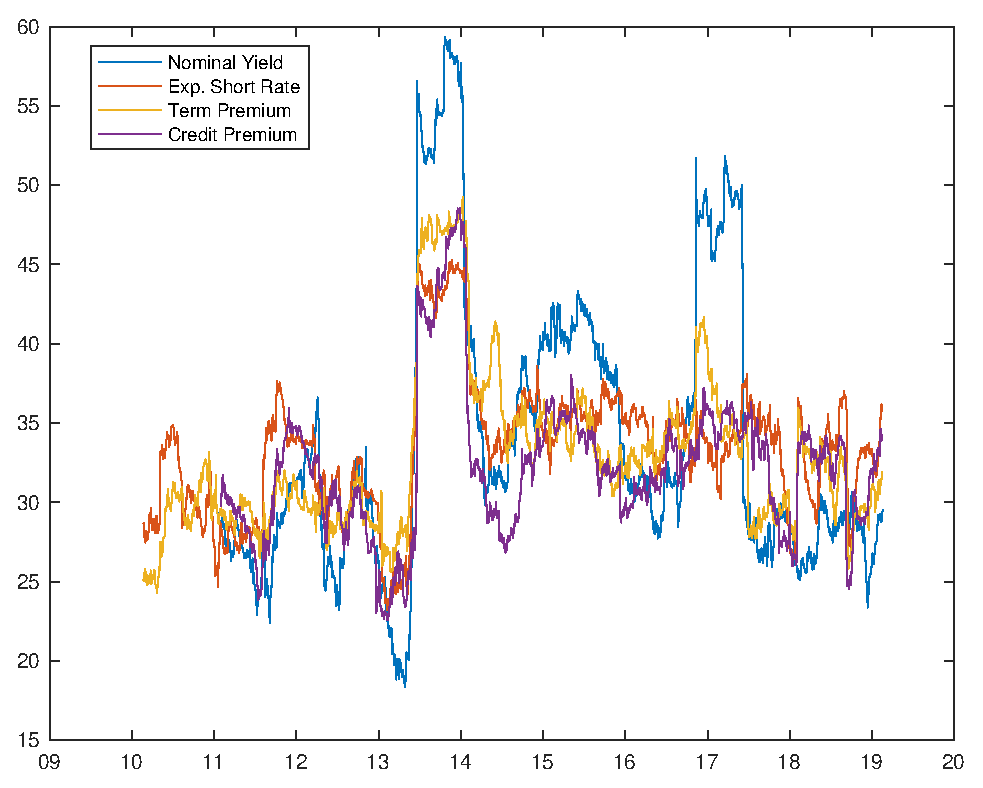
\includegraphics[trim={0cm 0cm 0cm 0cm},clip,height=0.34\textheight,width=\linewidth]{../Figures/Estimation/dy_index10y.eps} \\
			\vspace{-0.35cm}
			\caption{Emerging Markets} \label{subfig:dyindex10yEM}
			\vspace{0.4cm}
	\end{subfigure}
	
	\begin{subfigure}[t]{\linewidth}
			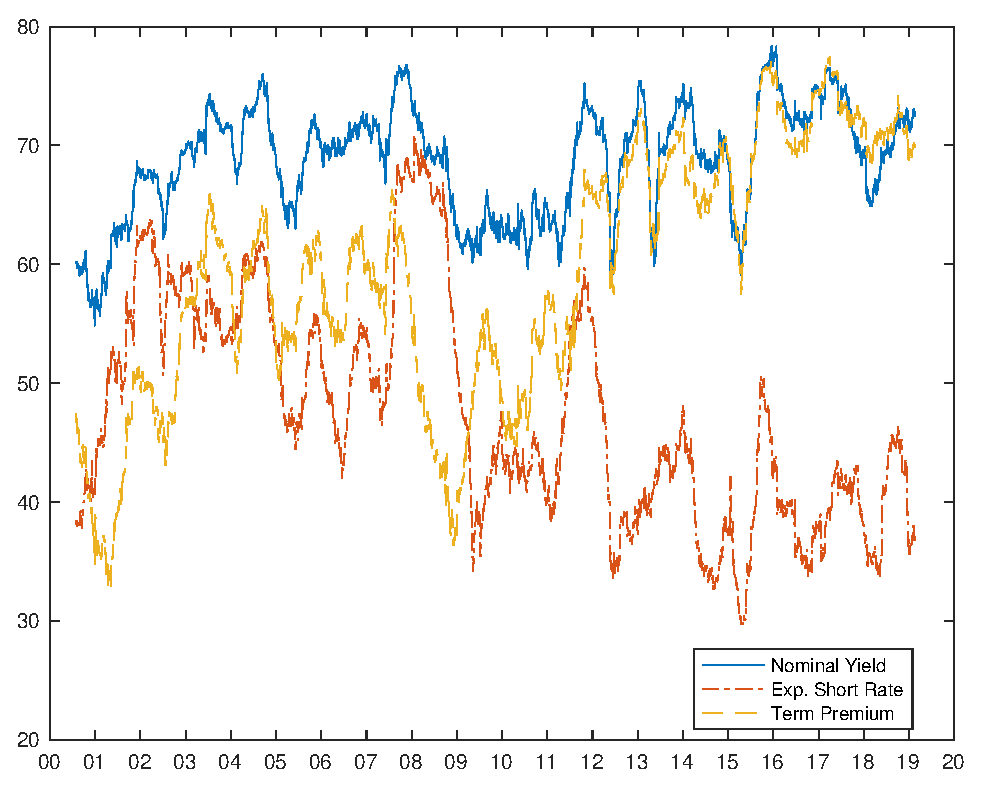
\includegraphics[trim={0cm 0cm 0cm 0cm},clip,height=0.34\textheight,width=\linewidth]{../Figures/Estimation/dy_index10y_AE.eps} \\
			\vspace{-0.35cm}
			\caption{Advanced Countries} \label{subfig:dyindex10yAE}
	\end{subfigure}
	\end{center}
	\fignotes{This figure plots the connected index of \cite{DieboldYilmaz:2014} for the 10-year nominal yields (solid line) of emerging markets and advanced countries. The figure also shows the index for each yield component. The yields of advanced countries are decomposed into an expected future short-term interest rate (line) and a term premium (line). The yields of emerging markets further have a credit risk premium (line). The index is obtained using a vector autoregression of order 1, with a forecast horizon of 10 days and a rolling window of 150 days for the daily changes of the 10-year nominal yields and each of their components. For emerging markets, the indexes have a shorter history because their computation requires a balanced panel; the indexes of the components do not start on the same date because the construction of the synthetic curves does not involve nominal yields.}
	\end{minipage}
\end{center}
\end{figure}
\end{document}
% trim = {<left> <lower> <right> <upper>}